\chapter{Équation de Schrödinger}

\paragraph{Exercice 1} \textit{Conservation des particules et courant de probabilité.} \\
On se donne une fonction d'onde $\Psi(t,\vec x)$ décrivant un système dynamique dans l'espace $\mathbb R^3$, solution de l'équation de Schrödinger 
\begin{equation}
\boxed{
-\frac{\hbar^2}{2m} \nabla^2 \Psi + V(\vec x) \Psi = i\hbar \frac{\partial\Psi}{\partial t}.
}
\end{equation}
Le module carré $|\Psi(t,\vec x)|^2$ de la fonction d'onde joue le même rôle que l'intensité pour les ondes classiques, mais doit être interprété ici comme la densité de probabilité de présence d'une particule à la position $\vec x$, à l'instant $t$. Nous allons montrer que l'équation de Schrödinger garantit la conservation de la particule au cours de son évolution. 
%Ceci suggère que lorsqu'une probabilité de présence diminue dans une région de l'espace, elle doit augmenter dans une autre, et un courant de probabilité s'est écoulé de la région que la particule quitte vers la région de destination. 
\begin{enumerate}
	\item Montrez que l'équation de Schrödinger peut se réécrire
	\begin{equation}
	\frac{\partial\rho}{\partial t} + \vec\nabla\cdot\vec J = 0
	\end{equation}
	où $\rho(t,\vec x) = |\Psi(t,\vec x)|^2$ et $\vec J(t,\vec x) = \frac{\hbar}{m} \text{Im}[\bar\Psi \vec \nabla \Psi]$. Donnez une signification physique à cette équation et aux quantités qu'elle implique. 
	\item Montrez que cela conduit à la conservation de la particule décrite par $\Psi(t,\vec x)$, et que la probabilité de présence dans l'espace complet est la norme de $\Psi(t,\vec x)$.
	%\item Sachant que l'on peut toujours écrire $\Psi(t,\vec x) = \sqrt{\rho(t,\vec x)} \, \exp i \theta(t,\vec x)$, montrez que $\vec  J(t,\vec x) = \rho(t,\vec x)\vec v(t,\vec x)$ et calculez $\vec v(t,\vec x)$. Quelle analogie vous est-elle suggérée par ce résultat ?
	%\item On se donne des champs $\rho(t,\vec x)$ et $\vec J(t,\vec x)$ arbitraires. Si l'on suppose qu'il existe un vecteur $\vec v(t,\vec x)$ tel que $\vec J = \rho\vec v$, montrez qu'il faut imposer que $\vec \nabla \times \vec v = \vec 0$ pour que l'on puisse associer la paire $(\rho,\vec J)$ à un état quantique $\Psi(t,\vec x)$. Donnez une expression générale pour le vecteur $\vec v$ en fonction de $\Psi(t,\vec x)$.
	\item On se donne des champs $\rho(t,\vec x)$ et $\vec J(t,\vec x)$ arbitraires. Montrez qu'une condition nécessaire et suffisante pour que ces champs décrivent un état physique $\Psi(t,\vec x)$ est $\vec\nabla\times (\vec J/\rho) = \vec 0$. Déduisez-en que deux états identiques peuvent différer par un facteur de phase global.
	\item Considérons une particule libre dont la quantité de mouvement $\vec p$ est \textit{parfaitement} connue. 
	\begin{enumerate}
	\item Écrivez la fonction d'onde $\Psi(t,\vec x)$ associée. 
	\item Calculez $\rho(t,\vec x)$, $J(t,\vec x)$ et interprétez vos résultats.
	\item Cette fonction d'onde est-elle de carré sommable ?
	\item Votre réponse vous surprend-elle ?
	\end{enumerate}
\end{enumerate}

\paragraph{Exercice 2} \textit{Propagation d'un paquet d'onde gaussien.} \\
Dans la réalité, la Relation de Heisenberg empêche quiconque de prédire exactement la position (respectivement l'impulsion) d'une particule sans provoquer l'indétermination totale de son impulsion (respectivement sa position). Imaginons qu'à l'origine du temps $t=0$ nous connaissions approximativement la position d'une particule autour de $x=0$, dont le mouvement sera supposé uni-dimensionnel et libre. L'incertitude sur cette position sera notée $L$. Nous pouvons représenter cette particule par une fonction d'onde gaussienne de largeur $L$ et d'impulsion initiale $p_0$ :
\begin{equation}
\Psi(0,x) = \frac{1}{\sqrt{L\sqrt{2\pi}}} e^{-\frac{x^2}{4L^2}} e^{\frac{i}{\hbar} p_0 x}.
\end{equation}	
Quelle sera la forme et la position du paquet d'onde en un instant futur $t>0$ ? C'est ce que nous allons déterminer.
\begin{enumerate}
\item Justifiez que la fonction d'onde peut généralement s'écrire comme une superposition d'ondes planes. Nous pouvons donc supposer que
\begin{equation}
\Psi(t,x) = \frac{1}{\sqrt{2\pi\hbar}} \int_{-\infty}^{+\infty} dp \, \psi(p) \, e^{\frac{i}{\hbar} (px - E(p) t)} 
\end{equation}
où les amplitudes $\psi(p)$ sont encore inconnues, et $E(p) = p^2/2m$. 
\item À l'aide de la forme de la fonction $\Psi(0,x)$, et de l'expression intégrale de la distribution de Dirac
\begin{equation}
\delta(p-p') = \frac{1}{2\pi\hbar} \int_{-\infty}^{+\infty} dx \, e^{\frac{i}{\hbar} (p-p')x},
\end{equation}
déterminez l'expression de $\psi(p)$. Calculez la moyenne statistique et l'écart-type de $\psi(p)$. Vérifiez que la Relation de Heisenberg est satisfaite.
\item Montrez que la fonction d'onde recherchée est donnée par
\begin{equation}
\Psi(t,x) = \frac{1}{(2\pi L^2 \beta^2)^{\frac{1}{4}} } e^{\frac{i}{\hbar}(p_0 x - E(p_0)t)} e^{-\frac{1}{4L^2\beta} (x - \frac{p_0}{m}t)^2}, \, \beta \equiv 1 + \frac{i\hbar t}{2mL^2}.
\end{equation}
\textit{Indication :} démontrez que
\begin{equation}
\int_{-\infty}^{+\infty} du \, e^{-\frac{u^2\alpha^2}{2}} e^{iuy} = \frac{\sqrt{2\pi}}{\alpha} e^{-\frac{y^2}{2\alpha^2}}
\end{equation}
pour $\alpha$ tel que $\text{Re}\lbrace \alpha^2\rbrace > 0$.
\item Calculez $\rho(t,x) = |\Psi(t,x)|^2$ et montrez qu'il s'agit aussi d'une distribution gaussienne, dont vous calculerez la moyenne statistique et l'écart-type. Interprétez vos résultats.
\item Calculez le courant de probabilité $J(t,x)$ associé à la propagation du paquet d'onde, et vérifiez que la particule est bien conservée.
\end{enumerate}

\paragraph{Exercice 3} \textit{Marche de potentiel.} \\
On considère une particule de masse $m$ en mouvement unidimensionnel le long de la direction $x$. Se déplaçant initialement dans la région $x<0$ de gauche à droite, elle rencontre en $x=0$ une marche de potentiel de hauteur finie et donnée par $V_0$. Nous analyserons deux cas distincts.
\begin{enumerate}
\item \textit{Réflexion partielle : $E > V_0$.} 
	\begin{enumerate}
		\item Justifiez qu'il n'existe aucun état propre d'énergie négative pour ce système.
		\item Résolvez l'équation de Schrödinger dans les régions $x>0$ et $x<0$.
		\item En guise de rafraîchissement de mémoire, montrez, comme vous l'avez vu au cours, que sous l'hypothèse d'un potentiel présentant une discontinuité finie en $x=0$ (ce qui est le cas ici !), la fonction d'onde de la particule ainsi que sa dérivée doivent être \textit{continues} en $x=0$.
		\item Faites bon usage de ces conditions de raccord pour trouver les probabilités de réflexion et transmission de la particule par la marche de potentiel. Commentez les résultats obtenus en les confrontant au cas classique.
	\end{enumerate}
\item \textit{Réflexion totale : $E < V_0$.}
	\begin{enumerate}
		\item Résolvez l'équation de Schrödinger dans les régions $x>0$ et $x<0$.
		\item Exigez la continuité de la fonction d'onde et de sa dérivée pour trouver les probabilités de réflexion et transmission de la particule par la marche de potentiel. 
		\item Supposons que vous soyez en mesure de photographier le système à un instant arbitrairement choisi. Est-il possible que la particule soit photographiée à \textit{droite} de la marche de potentiel ? Commentez.
		\item Calculez le déphasage entre l'onde incidente et l'onde réfléchie, et donnez-en une interprétation physique.
	\end{enumerate}
\end{enumerate}

\paragraph{Exercice 4} \textit{État lié dans un puits de potentiel infiniment mince.} \\
On considère une particule de masse $m$ en mouvement unidimensionnel le long de la direction $x$ et dont l'opérateur Hamiltonien est donné par
\begin{equation}
H = -\frac{\hbar^2}{2m} \frac{d^2}{dx^2} - \alpha \delta(x)
\end{equation}
où $\alpha$ est une constante réelle positive dont on donnera les dimensions.
\begin{enumerate}
\item Formez l'équation de Schrödinger qui décrit le mouvement de la particule. 
\item Intégrez-la autour du point ``dramatique'' $x=0$ sur un intervalle de rayon $\varepsilon >0$ quelconque fixé et arbitrairement proche de zéro. Montrez que la dérivée de la fonction d'onde $\Psi(x)$ subit une discontinuité en $x=0$ que vous exprimerez en fonction de $\alpha$, $m$ et $\Psi(0)$.
\item On suppose que l'énergie $E$ de la particule est négative (état lié). Résolvez l'équation de Schrödinger dans les régions $x<0$ et $x>0$.
%\begin{equation}
%\left\lbrace
%\begin{array}{ccc}
%x<0 & : & \Psi(x) = A_1 e^{\rho x} + A_1' e^{-\rho x} \\ 
%x>0 & : & \Psi(x) = A_2 e^{\rho x} + A_2' e^{-\rho x}
%\end{array} 
%\right.
%\end{equation}
%Déterminez la constante $\rho$ en fonction de $E$ et $m$.
\item Exigez les conditions de raccord en $x=0$ pour fixer les valeurs possibles pour l'énergie $E$, ainsi que les fonctions d'onde normées correspondantes.
\item Représentez graphiquement les fonctions d'onde déterminées au point précédent, et donnez un ordre de grandeur de leur largeur $\Delta x$. 
\end{enumerate}

\paragraph{Exercice 5} \textit{Transmission à travers une barrière de potentiel infiniment mince.} \\
On considère une particule de masse $m$ en mouvement unidimensionnel le long de la direction $x$ et dont l'opérateur Hamiltonien est à nouveau donné par
\begin{equation}
H = -\frac{\hbar^2}{2m} \frac{d^2}{dx^2} - \alpha \delta(x).
\end{equation}
On suppose qu'elle se propage de gauche à droite le long de la direction $x$ avec une énergie $E$ positive. 
\begin{enumerate}
\item Montrez qu'un état stationnaire de la particule peut s'écrire :
\begin{equation}
\left\lbrace
\begin{array}{ccl}
x<0 & : & \Psi(x) = e^{ikx} + A \, e^{-ikx} \\ 
x>0 & : & \Psi(x) = B \, e^{ikx}
\end{array} 
\right.
\end{equation}
où $k$, $A$ et $B$ sont des constantes dont vous calculerez la valeur en fonction de $E$, $m$ et $\alpha$. 
\item Posons $-E_L \equiv -m\alpha^2/2\hbar^2$, l'énergie de l'état lié de la particule. Calculez, en fonction du paramètre sans dimensions $\sigma = E/E_L$ les coefficients de réflexion et transmission de la barrière, notés respectivement $\mathcal{R}$ et $\mathcal{T}$.
\item Décrivez la variation de $\mathcal{R}$ et $\mathcal{T}$ en fonction de l'énergie incidente $E$. Que se passe-t-il lorsque $E\to+\infty$ ? Commentaires ?
\item Montrez que, si l'on prolonge l'expression de $\mathcal{T}$ pour des valeurs d'énergie négatives, elle diverge lorsque $E\to-E_L$. Commentaires ?
\end{enumerate}

\paragraph{Exercice 6} \textit{Piège quantique à murs infiniment minces.} \\
On considère une particule de masse $m$ en mouvement unidimensionnel le long de la direction $x$, dont l'énergie potentielle s'écrit
\begin{equation}
V(x) = -\alpha \delta(x)-\alpha \delta(x-\ell), \, \alpha>0,\, \ell >0.
\end{equation}
\begin{enumerate}
\item Calculez les états liés de la particule en fonction du paramètre $\rho$ défini implicitement par 
\begin{equation}
E = -\frac{\hbar^2\rho^2}{2m}.
\end{equation}
Montrez que les niveaux d'énergie possibles vérifient la relation
\begin{equation}
e^{-\rho\ell} = \pm \Big( 1 - \frac{2\rho}{\mu} \Big), \,\mu = \frac{2m\alpha}{\hbar^2}.
\end{equation}
Donnez une résolution graphique de cette équation.
\item Décrivez les états stationnaires du système.
	\begin{enumerate}
	\item \textit{État fondamental.} Montrez que l'état fondamental est pair, c'est-à-dire invariant par symétrie miroir par rapport au point central $x=\ell/2$. Montrez que son énergie $E_S$ est inférieure à l'énergie $-E_L$ de l'état lié introduite à l'exercice précédent. Donnez une interprétation physique pour ce résultat. Représentez graphiquement la fonction d'onde correspondante.
	\item \textit{État excité.} Montrez que, lorsque le puits est suffisamment large (au-delà d'une valeur critique pour $\ell$ que vous calculerez), il existe un état excité, impair cette fois, et d'énergie $E_A$ supérieure à $-E_L$. À nouveau, interprétez et représentez graphiquement la fonction d'onde correspondante.
	\end{enumerate}
\end{enumerate}

\paragraph{Exercice 7} \textit{Mouvement circulaire uniforme --- Modèle de Bohr.}  \\
Considérons une particule de masse $m$ confinée sur un cercle de rayon $R$ et de circonférence $L = 2\pi R$. Plus précisément, on admet qu'un potentiel confine la particule dans les directions transverses. Ce potentiel est tellement fort qu'aux échelles d'énergie que nous envisageons, le seul degré de liberté est le mouvement le long du cercle.\\

\begin{center}
    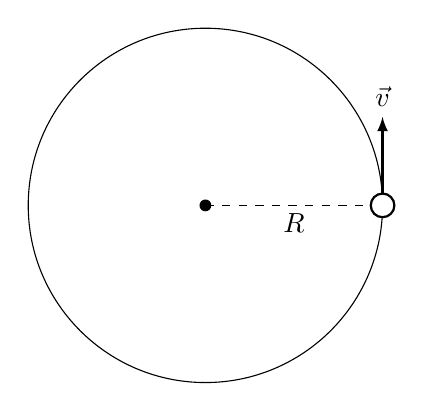
\begin{tikzpicture}[scale=0.75]
    \draw (2,2) circle (3cm);
    \fill (2,2) circle (0.1cm);
    \draw[dashed] (2,2) -- (5,2);
    \draw[-latex,thick] (5,2) -- (5,3.5)node[above]{$\vec v$};
    \draw[thick,fill=white] (5,2) circle (0.2cm);
    \node at (3.5,1.7) {$R$};
    \end{tikzpicture}
\end{center}
$ $\\
Soit $x \in [-\frac{L}{2},\frac{L}{2}]$ la coordonnée le long du cercle. L'origine $x=0$ est arbitrairement choisie, puisque ce système possède une symétrie de rotation.

\begin{enumerate}
    \item Quelles sont les conditions de raccord en $x= \pm \frac{L}{2}$ qu'il faut imposer sur $\psi(x)$ pour respecter la symétrie du problème ?
    \item Démontrez que les niveaux d'énergie de la particule sont quantifiés $\lbrace E_n\rbrace_{n\in\mathbb N}$, et déterminez les fonctions d'onde $\lbrace \varphi_n(x)\rbrace_{n\in\mathbb N}$ correspondantes. Les états sont-ils dégénérés ?
    \item Montrez que les fonctions d'onde associées à $m\neq n$ sont mutuellement orthogonales.
    \item Démontrez que le moment cinétique orbital de la particule est quantifié, $\mathcal L_n = \hbar n$.
    \end{enumerate}
    Le résultat précédent est en fait assez fondamental : le \textit{modèle de Bohr} de l'atome d'Hydrogène peut d'ailleurs être construit à partir de ce principe. Considérons un électron décrivant une orbite circulaire \textit{supposée} stable dans le potentiel électrostatique d'un proton, et faisons l'hypothèse que son moment cinétique orbital vérifie $\mathcal L = \hbar n$ où $n\in \mathbb N_0$. 
    \begin{enumerate}
    \setcounter{enumi}{4}
    \item Montrez que le rayon de cette orbite vérifie $R_n = a_0 n^2$ où $n\in\mathbb N_0$ et $a_0$ est le rayon de Bohr que l'on calculera. Comment pouviez-vous estimer la valeur de $a_0$ ?
    \item Quels sont, dans ce modèle, les niveaux d'énergie $\varepsilon_n$ de l'atome d'Hydrogène ? 
    \item Calculez la longueur d'onde dans le vide de la raie correspondant à la transition d'un électron du niveau $n'$ vers le niveau $n$ de l'atome d'Hydrogène (\textit{formule de Rydberg}). Quelle est l'énergie d'ionisation de cet atome ? 
\end{enumerate}

\newpage

\paragraph{Exercice 8} \textit{Boîte quantique avec barrière infiniment mince.} \hfill [\textit{Septembre 2019}] \\

Considérons une particule de masse $m$ confinée entre $x= -\frac{L}{2}$ et $x =+\frac{L}{2}$. En $x=0$ se trouve une barrière de potentiel suffisamment mince pour que nous puissions la représenter par une distribution $\delta$. \\

L'équation de Schrödinger stationnaire pour la particule est donc
\begin{equation}
-\frac{\hbar^2}{2m} \frac{d^2}{d x^2} \psi(x) + \alpha\, \delta(x)\, \psi(x)= E\, \psi(x)
\label{Eq:SchrDelta}
\end{equation}
avec $\alpha>0$ et les conditions aux bords $\psi(-\frac{L}{2})=0=\psi(+\frac{L}{2})$.

\begin{enumerate}
\item Quels sont les états stationnaires du système lorsque $\alpha = 0$. Calculez les niveaux d'énergie correspondants.

\item Dorénavant, nous considérons $\alpha \neq  0$. Quelles conditions de raccord faut-il imposer en $x=0$ pour tenir compte du potentiel $\delta$ ?

\item
Démontrez que toute solution de l'équation  \eqref{Eq:SchrDelta} possède une parité bien définie. Montrez en particulier que les fonctions d'onde impaires, solutions de l'équation \eqref{Eq:SchrDelta} avec $\alpha=0$ (trouvées au point 1), sont également solutions lorsque $\alpha\neq 0$ avec la même énergie.

\item Considérons à présent les solutions paires. En utilisant la condition de raccord dérivée au point 2, déterminez les niveaux d'énergie de ces solutions. 

\textit{Note :} Ces niveaux d'énergie seront donnés par une équation transcendante que vous ne pourrez pas résoudre analytiquement !
\end{enumerate}

\begin{figure}[h!]
    \centering
    \begin{tikzpicture}[scale=0.75]
    \draw[->] (-6,0) -- (6,0) node[right]{$x$};
    \draw[->] (-6,0) -- (-6,5) node[above]{$V$};
    \draw[very thick]  (-4,6) -- (-4,0);
    \draw  (-0.1, 4) -- (-0.1,0);
    \draw  (-0.1, 4) -- (0.1,4);
    \draw  (0.1, 4) -- (0.1,0);
    \draw[very thick]  (4,6) -- (4,0);
    %\node at (6,-0.5) {$x$};
    %\node at (-6.5,5) {$V$};
    \node at (-4,-0.5) {$-\frac{L}{2}$};
    \node at (0,-0.5) {$0$};
    \node at (4,-0.5) {$+\frac{L}{2}$};
    \node[above] at (0,4) {$\uparrow$};
    \node[above] at (0,4.6) {$\infty$};
    \fill[pattern=north east lines, pattern color=black] (4,0) rectangle (4.25,6);
    \fill[pattern=north west lines, pattern color=black] (-4,0) rectangle (-4.25,6);
    \end{tikzpicture}
    \caption{Représentation schématique du potentiel $V(x)$ de l'équation \eqref{Eq:SchrDelta}: $V$ est infini pour $x<-\frac{L}{2}$ et pour $x>\frac{L}{2}$. En outre un potentiel $\delta$ est présent en $x=0$.}
\end{figure}

\paragraph{Questions d'examen:} Juin 2019 Q4, Août 2019 Q4, Juin 2021 Q3, Août 2022 Q3.